\section{Casi d'uso}
Ogni caso d'uso identificato dall'analisi del capitolato C7, dagli incontri esterni con l'azienda IKS e dalle riunioni interne viene riportato in questa sezione attraverso un codice univoco gerarchico nella forma:
 $$ \textbf{UC \{codice\_padre\}.\{codice\_figlio\}  } $$
\begin{itemize}
	\item Le prime due lettere identificano che si tratta di un caso d'uso;
	\item Il codice padre è un numero univoco che identifica un caso d'uso;
	\item Il codice figlio è un numero progressivo che identifica i sottocasi;
\end{itemize}

\subsection{Attori}
Gli attori che interagiscono con il sistema sono:
\begin{itemize}
	\item \textbf{Utente}: ci si riferisce ad un utente generico che utilizza i due plugin già integrati su Kibana per monitorare ed analizzare le prestazioni di una determinata applicazione. 
	\item \textbf{Kibana}: piattaforma con cui i plugin devono interagire per reperire i dati da visualizzare in una forma specifica in seguito ad una richiesta da parte dell'utente.
\end{itemize}

\subsection{Caso d'uso UC1: Visualizzazione mappa topologica}
\begin{figure} [H]
	\centering
	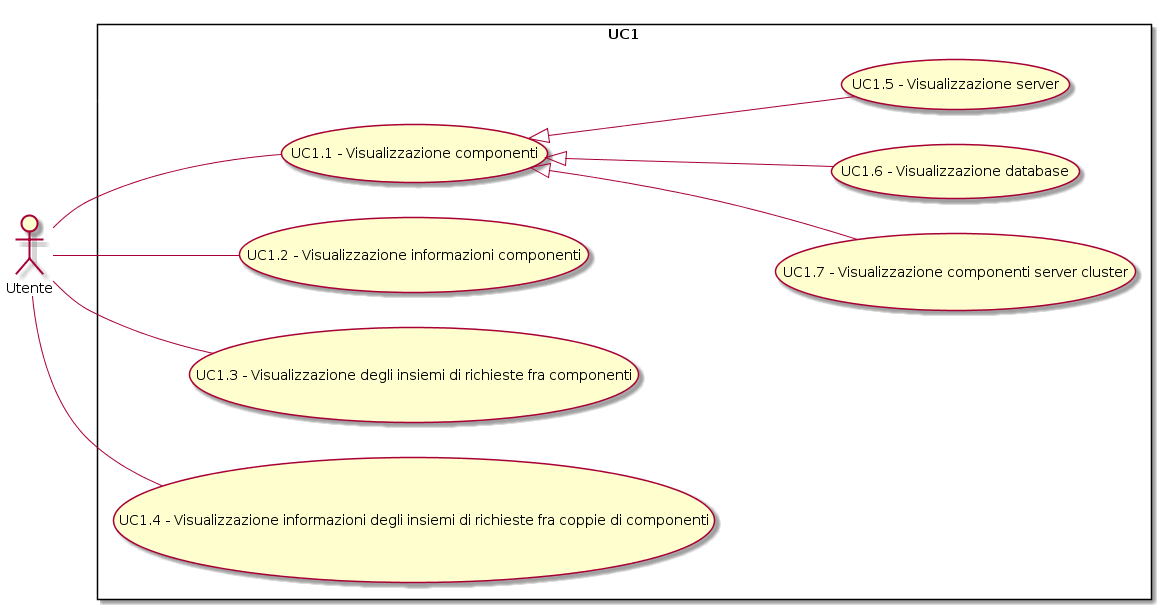
\includegraphics[scale=0.45]{./UC/UC1.png}
	\caption{Visualizzazione mappa topologica}\label{}
\end{figure}
\begin{itemize}
	\item \textbf{Attori}: Utente
	\item \textbf{Descrizione}: L'attore intende visualizzare la mappa topologica dell'applicazione monitorata.
	
	\item \textbf{Precondizione}: Kibana deve avere una dashboard che contenga il plugin della mappa.
	\item \textbf{Flusso principale degli eventi}: L'attore richiede di visualizzare la mappa dell'applicazione monitorata, il plugin carica ed elabora i dati relativi all'applicazione monitorata, il plugin mostra la mappa topologica dell'applicazione monitorata.
	\begin{itemize}
		\item Visualizzazione componenti (UC1.1)
		\item Visualizzazione informazioni componenti (UC1.2)
		\item Visualizzazione degli insiemi di richieste fra componenti (UC1.3)
		\item Visualizzazione informazioni degli insiemi di richieste fra coppie di componenti (UC1.4)
		\item Visualizzazione server (UC1.5)
		\item Visualizzazione database (UC1.6)
		\item Visualizzazione componenti server cluster (UC1.7)
	\end{itemize}
	\item \textbf{Postcondizione}: Viene mostrata la mappa topologica associata all'applicazione monitorata.
\end{itemize}
\subsection{Caso d'uso UC1.1: Visualizzazione componenti}
\begin{itemize}
	\item \textbf{Attori}: Utente
	\item \textbf{Descrizione}: L'attore intende visualizzare i componenti dell'applicazione monitorata.
	\item \textbf{Precondizione}: Kibana deve avere una dashboard che contenga il plugin della mappa.
	\item \textbf{Flusso principale degli eventi}: L'attore intende visualizzare i componenti dell'applicazione nella mappa, quindi essi vengono disegnati all'interno di essa.
	\item \textbf{Postcondizione}: I componenti vengono visualizzati all'interno della mappa.
\end{itemize}
\subsection{Caso d'uso UC1.2: Visualizzazione informazioni componenti}
\begin{figure} [H]
	\centering
	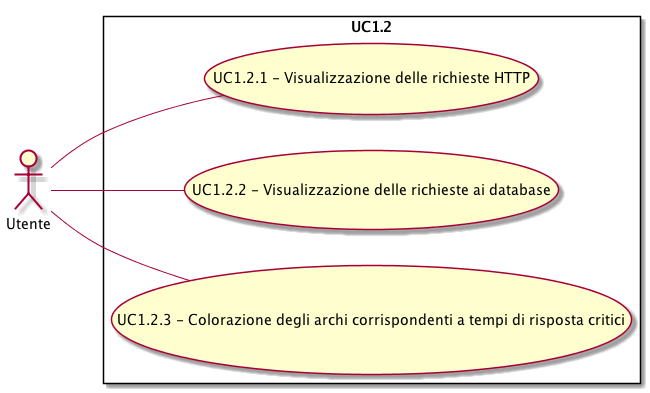
\includegraphics[scale=0.45]{./UC/UC1-2.png}
	\caption{Visualizzazione informazioni componenti}\label{}
\end{figure}
\begin{itemize}
	\item \textbf{Attori}: Utente
	\item \textbf{Descrizione}: L'attore intende visualizzare le informazioni dei componenti dell'applicazione monitorata.
	\item \textbf{Precondizione}: Kibana deve avere una dashboard che contenga il plugin della mappa.
	\item \textbf{Flusso principale degli eventi}: L'attore intende visualizzare le informazioni dei componenti dell'applicazione nella mappa, quindi esse vengono rappresentate all'interno di essa accanto al relativo componente.
	\begin{itemize}
		\item Visualizzazione del nome identificativo dei componenti (UC1.2.1)
		\item Visualizzazione del linguaggio di implementazione dei server (UC1.2.2)
	\end{itemize}
	\item \textbf{Postcondizione}: Le informazioni relative ad ogni componente vengono visualizzate sotto forma testuale accanto ad ognuno di essi.
\end{itemize}
\subsection{Caso d'uso UC1.2.1: Visualizzazione del nome identificativo dei componenti}
\begin{itemize}
	\item \textbf{Attori}: Utente
	\item \textbf{Descrizione}: L'attore intende visualizzare il nome di ciascun componente.
	\item \textbf{Precondizione}: Kibana deve avere una dashboard che contenga il plugin della mappa.
	\item \textbf{Flusso principale degli eventi}: L'attore intende visualizzare il nome identificativo di ogni componente presente nella mappa topologica che viene rappresentato accanto al componente.
	\item \textbf{Postcondizione}: Viene visualizzato vicino al componente il proprio nome identificativo sotto forma testuale.
\end{itemize}
\subsection{Caso d'uso UC1.2.2: Visualizzazione del linguaggio di implementazione dei server}
\begin{itemize}
	\item \textbf{Attori}: Utente
	\item \textbf{Descrizione}: L'attore intende visualizzare il linguaggio d'implementazione dei server.
	\item \textbf{Precondizione}: Kibana deve avere una dashboard che contenga il plugin della mappa.
	\item \textbf{Flusso principale degli eventi}: L'attore intende visualizzare il linguaggio di implementazione dei server presenti nella mappa topologica dell'applicazione, dunque essi vengono mostrati vicino al relativo server.
	\item \textbf{Postcondizione}: Viene visualizzato il linguaggio d'implementazione dei server presenti nella mappa topologica accanto ad ognuno di essi.
\end{itemize}
\subsection{Caso d'uso UC1.3: Visualizzazione degli insiemi di richieste fra componenti}
\begin{figure} [H]
	\centering
	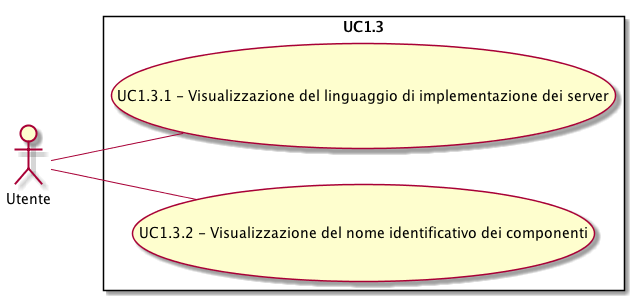
\includegraphics[scale=0.45]{./UC/UC1-3.png}
	\caption{Visualizzazione degli insiemi di richieste fra componenti}\label{}
\end{figure}
\begin{itemize}
	\item \textbf{Attori}: Utente
	\item \textbf{Descrizione}: L'attore intende visualizzare gli insiemi di richieste fra le coppie di componenti dell'applicazione monitorata sotto forma di archi.
	\item \textbf{Precondizione}: Kibana deve avere una dashboard che contenga il plugin della mappa.
	\item \textbf{Flusso principale degli eventi}: L'attore intende visualizzare gli insiemi di richieste fra coppie di componenti dell'applicazione nella mappa, quindi essi vengono disegnati all'interno di essa sotto forma di archi.
	\begin{itemize}
		\item Visualizzazione in base al tipo di richiesta (UC1.3.1)
		\item Colorazione degli archi corrispondenti a tempi di risposta (UC1.3.2)
		\item Visualizzazione delle richieste HTTP (UC1.3.3)
		\item Visualizzazione delle richieste ai database (UC1.3.4)
		\item Colorazione degli archi corrispondenti a tempi di risposta critici (UC1.3.5)
		\item Colorazione degli archi corrispondenti a tempi di risposta regolari (UC1.3.6)
	\end{itemize}
	\item \textbf{Postcondizione}: Gli insiemi di richieste fra coppie di componenti vengono visualizzate all'interno della mappa sotto forma di archi.
\end{itemize}
\subsection{Caso d'uso UC1.3.1: Visualizzazione in base al tipo di richiesta}
\begin{itemize}
	\item \textbf{Attori}: Utente
	\item \textbf{Descrizione}: L'attore intende visualizzare l'arco in base al tipo di richiesta eseguita fra le coppie di componenti dell'applicazione monitorata.
	\item \textbf{Precondizione}: Kibana deve avere una dashboard che contenga il plugin della mappa.
	\item \textbf{Flusso principale degli eventi}: L'attore intende visualizzare gli archi in base al tipo di richiesta fra coppie di componenti dell'applicazione nella mappa, quindi essi vengono disegnati all'interno di essa.
	\item \textbf{Postcondizione}: Vengono visualizzati gli archi in base al tipo di richiesta eseguita fra le coppie di componenti all'interno della mappa.
\end{itemize}
\subsection{Caso d'uso UC1.3.2: Colorazione degli archi corrispondenti a tempi di risposta}
\begin{itemize}
	\item \textbf{Attori}: Utente
	\item \textbf{Descrizione}: L'attore intende visualizzare gli insiemi di richieste fra le coppie di componenti dell'applicazione monitorata con colori diversi in base al loro tempo di esecuzione medio.
	\item \textbf{Precondizione}: Kibana deve avere una dashboard che contenga il plugin della mappa.
	
	\item \textbf{Flusso principale degli eventi}: L'attore intende visualizzare gli insiemi di richieste fra coppie di componenti con colori diversi in base al loro tempo medio di esecuzione, quindi essi vengono disegnati all'interno della mappa sotto forma di archi con il rispettivo colore.
	\item \textbf{Postcondizione}: Gli insiemi di richieste fra coppie di componenti vengono visualizzate all'interno della mappa sotto forma di archi di colore diverso in base al loro tempo di esecuzione medio.
\end{itemize}
\subsection{Caso d'uso UC1.3.3: Visualizzazione delle richieste HTTP}
\begin{itemize}
	\item \textbf{Attori}: Utente
	\item \textbf{Descrizione}: L'attore intende visualizzare gli insiemi di richieste HTTP fra le coppie di server dell'applicazione monitorata sotto forma di archi.
	\item \textbf{Precondizione}: Kibana deve avere una dashboard che contenga il plugin della mappa.
	\item \textbf{Flusso principale degli eventi}: L'attore intende visualizzare gli insiemi di richieste HTTP fra coppie di server dell'applicazione, quindi essi vengono disegnati all'interno della mappa sotto forma di archi.
	\item \textbf{Postcondizione}: Gli insiemi di richieste HTTP fra coppie di componenti vengono visualizzate all'interno della mappa sotto forma di archi.
\end{itemize}
\subsection{Caso d'uso UC1.3.4: Visualizzazione delle richieste ai database}
\begin{itemize}
	\item \textbf{Attori}: Utente
	\item \textbf{Descrizione}: L'attore intende visualizzare gli insiemi di richieste fatte fra coppie di server e database dell'applicazione monitorata sotto forma di archi fra i due componenti coinvolti.
	
	\item \textbf{Precondizione}: Kibana deve avere una dashboard che contenga il plugin della mappa.
	\item \textbf{Flusso principale degli eventi}: L'attore intende visualizzare gli insiemi di richieste fra coppie di server e database dell'applicazione, quindi essi vengono disegnati all'interno della mappa sotto forma di archi.
	\item \textbf{Postcondizione}: Gli insiemi di richieste fra coppie di server e database vengono visualizzate all'interno della mappa sotto forma di archi.
\end{itemize}
\subsection{Caso d'uso UC1.3.5: Colorazione degli archi corrispondenti a tempi di risposta critici}
\begin{itemize}
	\item \textbf{Attori}: Utente
	\item \textbf{Descrizione}: L'attore intende visualizzare gli insiemi di richieste fra le coppie di componenti dell'applicazione monitorata che hanno un tempo di esecuzione medio superiore a 3 secondi come archi rossi.
	
	\item \textbf{Precondizione}: Kibana deve avere una dashboard che contenga il plugin della mappa.
	\item \textbf{Flusso principale degli eventi}: L'attore intende visualizzare gli insiemi di richieste fra coppie di componenti che hanno un tempo medio di esecuzione superiore a 3 secondi di colore rosso, quindi essi vengono disegnati all'interno della mappa sotto forma di archi di colore rosso.
	\item \textbf{Postcondizione}: Gli insiemi di richieste fra coppie di componenti che hanno un tempo di esecuzione medio superiore a 3 secondi vengono visualizzate all'interno della mappa sotto forma di archi di colore rosso.
\end{itemize}
\subsection{Caso d'uso UC1.3.6: Colorazione degli archi corrispondenti a tempi di risposta regolari}
\begin{itemize}
	\item \textbf{Attori}: Utente
	\item \textbf{Descrizione}: L'attore intende visualizzare gli insiemi di richieste fra le coppie di componenti dell'applicazione monitorata che hanno un tempo di esecuzione medio inferiore o uguale a 3 secondi come archi neri.
	\item \textbf{Precondizione}: Kibana deve avere una dashboard che contenga il plugin della mappa.
	\item \textbf{Flusso principale degli eventi}: L'attore intende visualizzare gli insiemi di richieste fra coppie di componenti che hanno un tempo medio di esecuzione inferiore o uguale a 3 secondi di colore nero, quindi essi vengono disegnati all'interno della mappa sotto forma di archi di colore nero.
	\item \textbf{Postcondizione}: Gli insiemi di richieste fra coppie di componenti che hanno un tempo di esecuzione medio inferiore o uguale a 3 secondi vengono visualizzate all'interno della mappa sotto forma di archi di colore nero.
\end{itemize}
\subsection{Caso d'uso UC1.4: Visualizzazione informazioni degli insiemi di richieste fra coppie di componenti}
\begin{figure} [H]
	\centering
	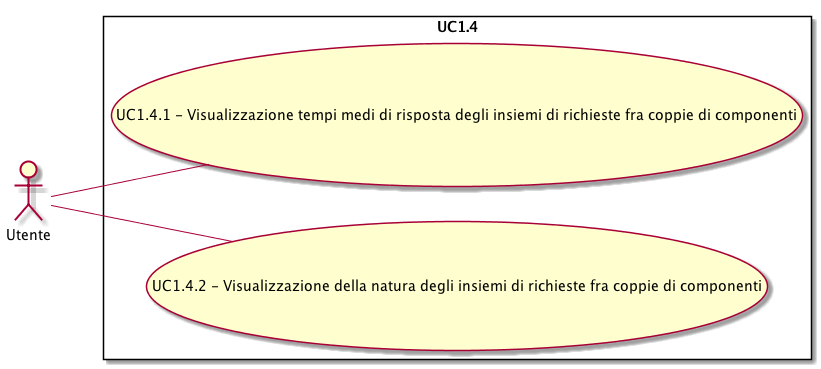
\includegraphics[scale=0.45]{./UC/UC1-4.png}
	\caption{Visualizzazione informazioni degli insiemi di richieste fra coppie di componenti}\label{}
\end{figure}
\begin{itemize}
	\item \textbf{Attori}: Utente
	\item \textbf{Descrizione}: L'attore intende visualizzare le informazioni relative a ciascun insieme di richieste fra coppie di componenti dell'applicazione monitorata.
	\item \textbf{Precondizione}: Kibana deve avere una dashboard che contenga il plugin della mappa.
	\item \textbf{Flusso principale degli eventi}: L'attore intende visualizzare le informazioni relative a ciascun insieme di richieste fra coppie di componenti dell'applicazione, quindi esse vengono rappresentate all'interno della mappa sotto forma di testo vicino al relativo arco.
	\begin{itemize}
		\item Visualizzazione tempi medi di risposta degli insiemi di richieste fra coppie di componenti (UC1.4.1)
		\item Visualizzazione della natura degli insiemi di richieste fra coppie di componenti (UC1.4.2)
	\end{itemize}
	\item \textbf{Postcondizione}: Le informazioni relative a ciascun insieme di richieste fra coppie di componenti vengono visualizzate all'interno della mappa.
\end{itemize}
\subsection{Caso d'uso UC1.4.1: Visualizzazione tempi medi di risposta degli insiemi di richieste fra coppie di componenti}
\begin{itemize}
	\item \textbf{Attori}: Utente
	\item \textbf{Descrizione}: L'attore intende visualizzare i tempi medi di risposta relativi a ciascun insieme di richieste fra coppie di componenti dell'applicazione monitorata.
	
	\item \textbf{Precondizione}: Kibana deve avere una dashboard che contenga il plugin della mappa.
	\item \textbf{Flusso principale degli eventi}: L'attore intende visualizzare i tempi medi di risposta di ciascun insieme di richieste fra coppie di componenti dell'applicazione, quindi essi vengono rappresentati all'interno di essa sotto forma di testo vicino al relativo arco.
	\item \textbf{Postcondizione}: I tempi medi di risposta relativi a ciascun insieme di richieste fra coppie di componenti vengono visualizzati all'interno della mappa vicino al relativo arco che rappresenta l'insieme di richieste.
\end{itemize}
\subsection{Caso d'uso UC1.4.2: Visualizzazione della natura degli insiemi di richieste fra coppie di componenti}
\begin{figure} [H]
	\centering
	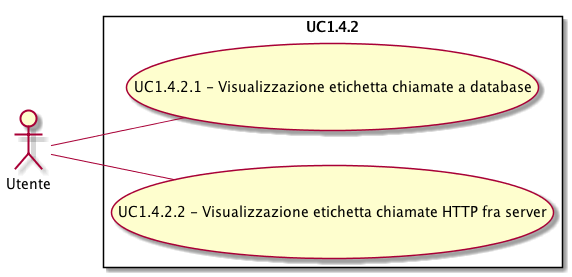
\includegraphics[scale=0.45]{./UC/UC1-4-2.png}
	\caption{Visualizzazione della natura degli insiemi di richieste fra coppie di componenti}\label{}
\end{figure}
\begin{itemize}
	\item \textbf{Attori}: Utente
	\item \textbf{Descrizione}: L'attore intende visualizzare le nature di ciascun insieme di richieste fra coppie di componenti dell'applicazione monitorata.
	\item \textbf{Precondizione}: Kibana deve avere una dashboard che contenga il plugin della mappa.
	
	\item \textbf{Flusso principale degli eventi}: L'attore intende visualizzare le nature di ciascun insieme di richieste fra coppie di componenti dell'applicazione, quindi esse vengono rappresentate all'interno della mappa sotto forma di etichetta vicino al relativo arco.
	\begin{itemize}
		\item Visualizzazione etichetta chiamate a database (UC1.4.2.1)
		\item Visualizzazione etichetta chiamate HTTP fra server (UC1.4.2.2)
	\end{itemize}
	\item \textbf{Postcondizione}: Le nature relative a ciascun insieme di richieste fra coppie di componenti vengono visualizzate all'interno della mappa vicino al relativo arco che rappresenta l'insieme di richieste.
\end{itemize}
\subsection{Caso d'uso UC1.4.2.1: Visualizzazione etichetta chiamate a database}
\begin{itemize}
	\item \textbf{Attori}: Utente
	\item \textbf{Descrizione}: L'attore intende visualizzare un'etichetta vicino ad ogni arco rappresentante un insieme di richieste da un server ad un database con testo "DB".
	\item \textbf{Precondizione}: Kibana deve avere una dashboard che contenga il plugin della mappa.
	
	\item \textbf{Flusso principale degli eventi}: L'attore intende visualizzare delle etichette con testo "DB" vicino ad ogni arco che rappresenti un insieme di richieste fra server e database, dunque tali etichette vengono disegnate.
	\item \textbf{Postcondizione}: Vengono disegnate sulla mappa, vicino ad ogni arco che rappresenti un insieme di richieste da server a database, delle etichette con testo "DB".
\end{itemize}
\subsection{Caso d'uso UC1.4.2.2: Visualizzazione etichetta chiamate HTTP fra server}
\begin{itemize}
	\item \textbf{Attori}: Utente
	\item \textbf{Descrizione}: L'attore intende visualizzare un'etichetta vicino ad ogni arco rappresentante un insieme di richieste HTTP da un server ad un altro server con testo "HTTP".
	\item \textbf{Precondizione}: Kibana deve avere una dashboard che contenga il plugin della mappa.
	\item \textbf{Flusso principale degli eventi}: L'attore intende visualizzare delle etichette con testo "HTTP" vicino ad ogni arco che rappresenti un insieme di richieste HTTP fra server e server, dunque tali etichette vengono disegnate.
	\item \textbf{Postcondizione}: Vengono disegnate sulla mappa, vicino ad ogni arco che rappresenti un insieme di richieste HTTP da server ad un altro server, delle etichette con testo "HTTP".
	
\end{itemize}
\subsection{Caso d'uso UC1.5: Visualizzazione server}
\begin{figure} [H]
	\centering
	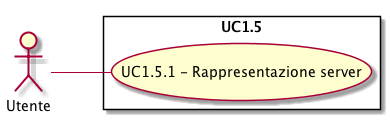
\includegraphics[scale=0.45]{./UC/UC1-5.png}
	\caption{Visualizzazione server}\label{}
\end{figure}
\begin{itemize}
	\item \textbf{Attori}: Utente
	\item \textbf{Descrizione}: L'attore intende visualizzare nella mappa topologica i server presenti nell'applicazione monitorata.
	\item \textbf{Precondizione}: Kibana deve avere una dashboard che contenga il plugin della mappa.
	
	\item \textbf{Flusso principale degli eventi}: L'attore intende visualizzare i server presenti nell'applicazione monitorata, essi vengono quindi disegnati all'interno della mappa.
	\begin{itemize}
		\item Rappresentazione server (UC1.5.1)
	\end{itemize}
	\item \textbf{Postcondizione}: Vengono mostrati i server nella mappa topologica dell'applicazione monitorata.
\end{itemize}
\subsection{Caso d'uso UC1.5.1: Rappresentazione server}
\begin{itemize}
	\item \textbf{Attori}: Utente
	\item \textbf{Descrizione}: L'attore intende visualizzare nella mappa topologica, per ogni server un cerchio che lo rappresenti.
	\item \textbf{Precondizione}: Kibana deve avere una dashboard che contenga il plugin della mappa.
	\item \textbf{Flusso principale degli eventi}: L'attore intende visualizzare i server presenti nell'applicazione monitorata, dunque per ciascuno di essi viene disegnato un cerchio che lo rappresenti.
	\item \textbf{Postcondizione}: Ogni server presente nella mappa viene rappresentato mediante un cerchio.
\end{itemize}
\subsection{Caso d'uso UC1.6: Visualizzazione database}
\begin{figure} [H]
	\centering
	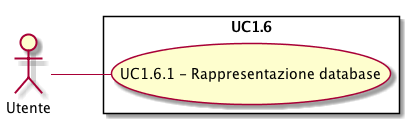
\includegraphics[scale=0.45]{./UC/UC1-6.png}
	\caption{Visualizzazione database}\label{}
\end{figure}
\begin{itemize}
	\item \textbf{Attori}: Utente
	\item \textbf{Descrizione}: L'attore intende visualizzare nella mappa topologica i database presenti nell'applicazione monitorata.
	\item \textbf{Precondizione}: Kibana deve avere una dashboard che contenga il plugin della mappa.
	\item \textbf{Flusso principale degli eventi}: L'attore intende visualizzare i database presenti nell'applicazione monitorata, essi vengono quindi disegnati all'interno della mappa.
	\begin{itemize}
		\item Rappresentazione database (UC1.6.1)
	\end{itemize}
	\item \textbf{Postcondizione}: Vengono mostrati i database nella mappa topologica dell'applicazione monitorata.
\end{itemize}
\subsection{Caso d'uso UC1.6.1: Rappresentazione database}
\begin{itemize}
	\item \textbf{Attori}: Utente
	\item \textbf{Descrizione}: L'attore intende visualizzare nella mappa topologica, per ogni database un cilindro che lo rappresenti.
	\item \textbf{Precondizione}: Kibana deve avere una dashboard che contenga il plugin della mappa.
	\item \textbf{Flusso principale degli eventi}: L'attore intende visualizzare i database presenti nell'applicazione monitorata, dunque per ciascuno di essi viene disegnato un cilindro che lo rappresenti.
	
	\item \textbf{Postcondizione}: Ogni database presente nella mappa viene rappresentato mediante un cilindro.
\end{itemize}
\subsection{Caso d'uso UC1.7: Visualizzazione componenti server cluster}
\begin{figure} [H]
	\centering
	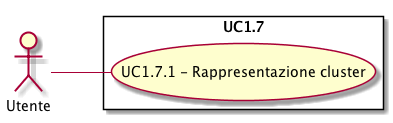
\includegraphics[scale=0.45]{./UC/UC1-7.png}
	\caption{Visualizzazione componenti server cluster}\label{}
\end{figure}
\begin{itemize}
	\item \textbf{Attori}: Utente
	\item \textbf{Descrizione}: L'attore intende visualizzare nella mappa topologica i server cluster presenti nell'applicazione monitorata.
	\item \textbf{Precondizione}: Kibana deve avere una dashboard che contenga il plugin della mappa.
	\item \textbf{Flusso principale degli eventi}: L'attore intende visualizzare i server cluster presenti nell'applicazione monitorata, essi vengono quindi disegnati all'interno della mappa.
	\begin{itemize}
		\item Rappresentazione cluster (UC1.7.1)
	\end{itemize}
	\item \textbf{Postcondizione}: Vengono mostrati i server cluster nella mappa topologica dell'applicazione monitorata.
\end{itemize}
\subsection{Caso d'uso UC1.7.1: Rappresentazione cluster}
\begin{itemize}
	\item \textbf{Attori}: Utente
	\item \textbf{Descrizione}: L'attore intende visualizzare nella mappa topologica, per ogni server cluster il numero di server che lo compongono.
	\item \textbf{Precondizione}: Kibana deve avere una dashboard che contenga il plugin della mappa.
	\item \textbf{Flusso principale degli eventi}: L'attore intende visualizzare il numero di server che compongono ciascun server cluster presente nell'applicazione monitorata, dunque per ciascuno di essi viene disegnato il numero di server di cui è composto.
	\item \textbf{Postcondizione}: Per ogni server cluster presente nella mappa viene visualizzato il relativo numero di server che lo compongono.
\end{itemize}
\subsection{Caso d'uso UC2: Riposizionamento componenti della mappa topologica}
\begin{figure} [H]
	\centering
	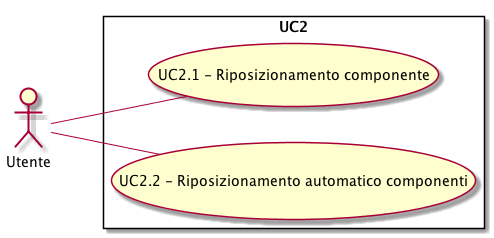
\includegraphics[scale=0.45]{./UC/UC2.png}
	\caption{Riposizionamento componenti della mappa topologica}\label{}
\end{figure}
\begin{itemize}
	\item \textbf{Attori}: Utente
	\item \textbf{Descrizione}: L'attore intende riposizionare i componenti della mappa topologica.
	\item \textbf{Precondizione}: Deve essere visualizzata la mappa topologica dell'applicazione monitorata.
	\item \textbf{Flusso principale degli eventi}: L'attore interagisce con le componenti grafiche dedicate alla manipolazione della mappa topologica e modifica il posizionamento dei componenti all'interno di essa.
	\begin{itemize}
		\item Riposizionamento componente (UC2.1)
		\item Riposizionamento automatico componenti (UC2.2)
	\end{itemize}
	\item \textbf{Postcondizione}: La visualizzazione della mappa topologica risulta modificata come nelle intenzioni dell'attore.
\end{itemize}
\subsection{Caso d'uso UC2.1: Riposizionamento componente}
\begin{itemize}
	\item \textbf{Attori}: Utente
	\item \textbf{Descrizione}: L'attore intende spostare un componente all'interno della mappa topologica dell'applicazione monitorata.
	\item \textbf{Precondizione}: Deve essere stato caricato da Kibana il plugin della mappa topologica dell'applicazione.
	\item \textbf{Flusso principale degli eventi}: L'attore trascina un componente della mappa topologica con il puntatore Il componente trascinato viene riposizionato.
	\item \textbf{Postcondizione}: Il componente trascinato viene riposizionato.
\end{itemize}
\subsection{Caso d'uso UC2.2: Riposizionamento automatico componenti}
\begin{itemize}
	\item \textbf{Attori}: Utente
	\item \textbf{Descrizione}: L'attore intende riposizionare tutti i componenti della mappa topologica dell'applicazione monitorata in modo automatico.
	\item \textbf{Precondizione}: Deve essere stato caricato da Kibana il plugin della mappa topologica dell'applicazione e qualche componente deve essere già stato riposizionato.
	\item \textbf{Flusso principale degli eventi}: L'attore preme un componente grafico che avvii il riposizionamento delle componenti Le componenti che sono state spostate vengono riposizionate nella loro posizione iniziale.
	\item \textbf{Postcondizione}: Tutti i componenti della mappa si trovano nella posizione iniziale in cui è stata caricata la mappa.
\end{itemize}
\subsection{Caso d'uso UC3: Ridimensionamento della mappa topologica}
\begin{figure} [H]
	\centering
	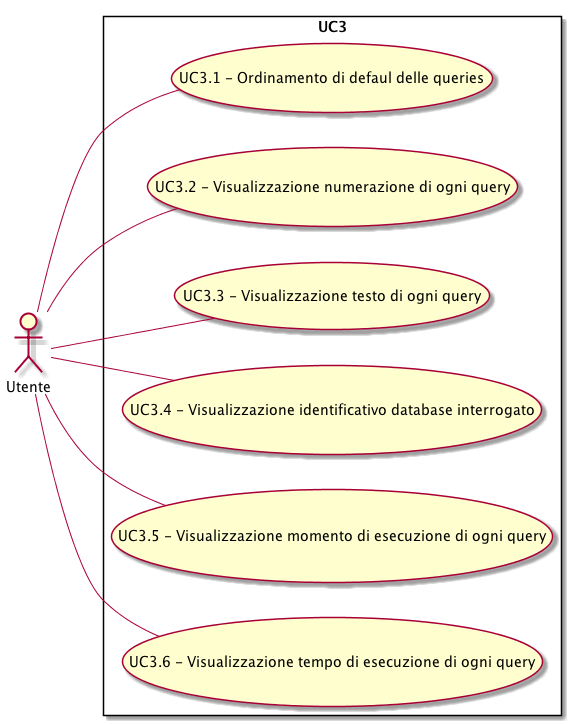
\includegraphics[scale=0.45]{./UC/UC3.png}
	\caption{Ridimensionamento della mappa topologica}\label{}
\end{figure}
\begin{itemize}
	\item \textbf{Attori}: Utente
	\item \textbf{Descrizione}: L'attore intende eseguire un ridimensionamento della mappa topologica.
	\item \textbf{Precondizione}: Deve essere stato caricato il plugin della mappa topologica.
	\item \textbf{Flusso principale degli eventi}: L'attore interagisce con un componente grafico che permetta il ridimensionamento della mappa, quindi essa viene ridimensionata.
	\begin{itemize}
		\item Ingrandimento della mappa topologica (UC3.1)
		\item Restringimento della mappa (UC3.2)
		\item Visualizzazione mappa a schermo intero (UC3.3)
	\end{itemize}
	\item \textbf{Postcondizione}: La mappa topologica viene ridimensionata.
\end{itemize}
\subsection{Caso d'uso UC3.1: Ingrandimento della mappa topologica}
\begin{itemize}
	\item \textbf{Attori}: Utente
	\item \textbf{Descrizione}: L'attore intende ingrandire la rappresentazione grafica della mappa.
	\item \textbf{Precondizione}: Deve essere stato caricato il plugin della mappa topologica dell'applicazione.
	\item \textbf{Flusso principale degli eventi}: L'attore preme un componente grafico che permetta l'ingrandimento della mappa. La mappa viene quindi ingrandita.
	\item \textbf{Postcondizione}: La mappa viene ingrandita.
\end{itemize}
\subsection{Caso d'uso UC3.2: Restringimento della mappa}
\begin{itemize}
	\item \textbf{Attori}: Utente
	\item \textbf{Descrizione}: L'attore intende restringere la rappresentazione grafica della mappa.
	\item \textbf{Precondizione}: Deve essere stato caricato il plugin della mappa topologica dell'applicazione.
	\item \textbf{Flusso principale degli eventi}: L'attore preme un componente grafico che permetta la restrizione della mappa topologica, la rappresentazione della mappa viene ristretta.
	\item \textbf{Postcondizione}: La rappresentazione della mappa viene ristretta.
\end{itemize}
\subsection{Caso d'uso UC3.3: Visualizzazione mappa a schermo intero}
\begin{itemize}
	\item \textbf{Attori}: Utente
	\item \textbf{Descrizione}: L'attore intende visualizzare la mappa a schemo intero.
	\item \textbf{Precondizione}: Deve essere stata caricata la mappa topologica dell'applicazione monitorata.
	\item \textbf{Flusso principale degli eventi}: L'attore preme sul componente grafico dedicato all'attivazione della modalità a schermo interro ed essa viene visualizzata schermo intero.
	\item \textbf{Postcondizione}: La mappa topologica viene visualizzata a schermo intero.
\end{itemize}
\subsection{Caso d'uso UC4: Fallimento caricamento dati della mappa topologica}
\begin{itemize}
	\item \textbf{Attori}: Utente
	\item \textbf{Descrizione}: I dati relativi alla mappa topologica non possono essere caricati per un errore interno.
	
	\item \textbf{Precondizione}: Si verifica un errore nel caricamento dei dati.
	\item \textbf{Flusso principale degli eventi}: La richiesta dei dati relativi alla mappa topologica dell'applicazione monitorata non può essere soddisfatta, dunque viene visualizzato un messaggio di errore al posto della mappa.
	\item \textbf{Postcondizione}: Al posto della mappa topologica viene visualizzato un messaggio di errore.
\end{itemize}
\subsection{Caso d'uso UC5: Visualizzazione stack trace}
\begin{figure} [H]
	\centering
	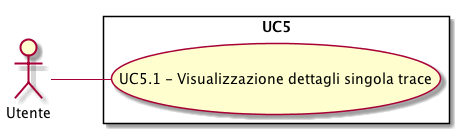
\includegraphics[scale=0.45]{./UC/UC5.png}
	\caption{Visualizzazione stack trace}\label{}
\end{figure}
\begin{itemize}
	\item \textbf{Attori}: Utente
	\item \textbf{Descrizione}: L'attore intende visualizzare la lista delle trace dell'applicazione monitorata.
	\item \textbf{Precondizione}: Kibana deve avere una dashboard che contenga il plugin della stack trace.
	\item \textbf{Flusso principale degli eventi}: L'attore intende visualizzare la lista delle trace dell'applicazione monitorata, il plugin carica ed elabora i dati relativi alle trace, dunque mostra all'attore la lista delle trace.
	\begin{itemize}
		\item Visualizzazione dettagli singola trace (UC5.1)
	\end{itemize}
	\item \textbf{Postcondizione}: Viene mostrato l'elenco delle trace.
\end{itemize}
\subsection{Caso d'uso UC5.1: Visualizzazione dettagli singola trace}
\begin{figure} [H]
	\centering
	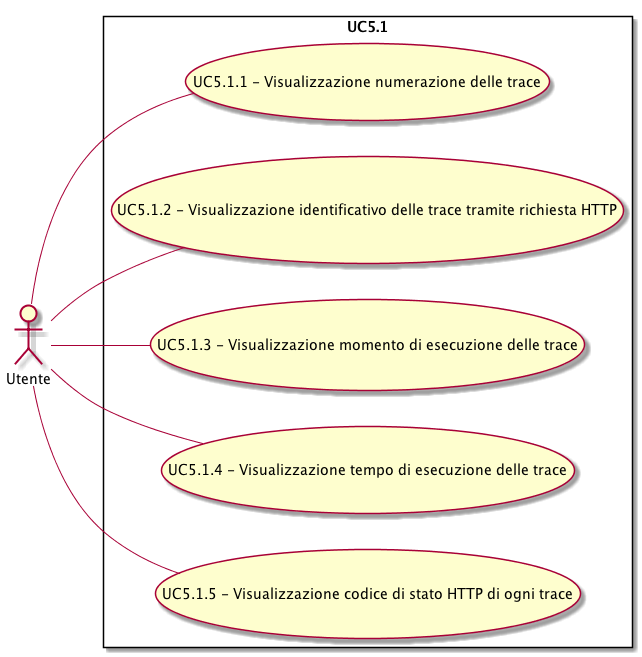
\includegraphics[scale=0.45]{./UC/UC5-1.png}
	\caption{Visualizzazione dettagli singola trace}\label{}
\end{figure}
\begin{itemize}
	\item \textbf{Attori}: Utente
	\item \textbf{Descrizione}: L'attore intende visualizzare, per ogni trace, i dettagli disponibili.
	\item \textbf{Precondizione}: Kibana deve avere una dashboard che contenga il plugin della stack trace.
	\item \textbf{Flusso principale degli eventi}: L'attore intende visualizzare, per ogni trace, i relativi dettagli che vengono visualizzati e raggruppati in una riga della lista.
	\begin{itemize}
		\item Visualizzazione numerazione delle trace (UC5.1.1)
		\item Visualizzazione identificativo delle trace tramite richiesta HTTP (UC5.1.2)
		\item Visualizzazione momento di esecuzione delle trace (UC5.1.3)
		\item Visualizzazione tempo di esecuzione delle trace (UC5.1.4)
		\item Visualizzazione codice di stato HTTP di ogni trace (UC5.1.5)
	\end{itemize}
	\item \textbf{Postcondizione}: Vengono visualizzati i dettagli relativi ad ogni singola query.
\end{itemize}
\subsection{Caso d'uso UC5.1.1: Visualizzazione numerazione delle trace}
\begin{itemize}
	\item \textbf{Attori}: Utente
	\item \textbf{Descrizione}: L'attore intende visualizzare la lista delle trace come un elenco numerato che parta da 1.
	\item \textbf{Precondizione}: Kibana deve avere una dashboard che contenga il plugin della lista delle trace.
	\item \textbf{Flusso principale degli eventi}: L'attore intende visualizzare la lista delle trace come un elenco numerato, quindi vicino ad ogni trace viene disegnato un numero incrementale che parte da 1.
	\item \textbf{Postcondizione}: La lista delle trace viene visualizzata come un elenco numerato.
\end{itemize}
\subsection{Caso d'uso UC5.1.2: Visualizzazione identificativo delle trace tramite richiesta HTTP}
\begin{itemize}
	\item \textbf{Attori}: Utente
	\item \textbf{Descrizione}: L'attore intende visualizzare le trace identificandole con la richiesta HTTP effettuata da ognuna di esse.
	\item \textbf{Precondizione}: Kibana deve avere una dashboard che contenga il plugin della stack trace.
	\item \textbf{Flusso principale degli eventi}: L'attore intende visualizzare la lista delle trace tramite la richiesta HTTP effettuata da ognuna di esse, che viene visualizzata in forma testuale.
	\item \textbf{Postcondizione}: Ogni trace presente nella lista viene visualizzata con il proprio identificativo dato dalla richiesta HTTP effettuata.
\end{itemize}
\subsection{Caso d'uso UC5.1.3: Visualizzazione momento di esecuzione delle trace}
\begin{itemize}
	\item \textbf{Attori}: Utente
	\item \textbf{Descrizione}: L'attore intende visualizzare data e orario del momento in cui è iniziata l'esecuzione di ogni trace.
	\item \textbf{Precondizione}: Kibana deve avere una dashboard che contenga il plugin della stack trace.
	\item \textbf{Flusso principale degli eventi}: L'attore intende visualizzare data e orario del momento in cui è iniziata l'esecuzione di ogni trace dunque tali informazioni vengono rappresentate in maniera testuale.
	\item \textbf{Postcondizione}: Vengono mostrate la data e l'orario del momento in cui è iniziata l'esecuzione di ogni trace.
\end{itemize}
\subsection{Caso d'uso UC5.1.4: Visualizzazione tempo di esecuzione delle trace}
\begin{itemize}
	\item \textbf{Attori}: Utente
	\item \textbf{Descrizione}: L'attore intende visualizzare il tempo di esecuzione di ogni trace.
	\item \textbf{Precondizione}: Kibana deve avere una dashboard che contenga il plugin della stack trace.
	\item \textbf{Flusso principale degli eventi}: L'attore intende visualizzare il tempo di esecuzione di ogni trace ed esso viene rappresentato sotto forma di testo.
	\item \textbf{Postcondizione}: Per ogni trace presente nella lista viene visualizzato il proprio tempo di esecuzione.
\end{itemize}
\subsection{Caso d'uso UC5.1.5: Visualizzazione codice di stato HTTP di ogni trace}
\begin{figure} [H]
	\centering
	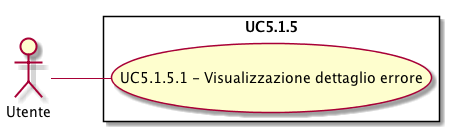
\includegraphics[scale=0.45]{./UC/UC5-1-5.png}
	\caption{Visualizzazione codice di stato HTTP di ogni trace}\label{}
\end{figure}
\begin{itemize}
	\item \textbf{Attori}: Utente
	\item \textbf{Descrizione}: L'attore intende visualizzare il codice di stato HTTP associato ad ogni trace.
	\item \textbf{Precondizione}: Kibana deve avere una dashboard che contenga il plugin della stack trace.
	\item \textbf{Flusso principale degli eventi}: L'attore intende visualizzare il codice di stato HTTP di ogni trace ed esso viene rappresentato sotto forma di testo.
	\begin{itemize}
		\item Visualizzazione dettaglio errore (UC5.1.5.1)
	\end{itemize}
	\item \textbf{Postcondizione}: Per ogni trace presente nella lista viene visualizzato il proprio codice di stato HTTP.
\end{itemize}
\subsection{Caso d'uso UC5.1.5.1: Visualizzazione dettaglio errore}
\begin{itemize}
	\item \textbf{Attori}: Utente
	\item \textbf{Descrizione}: L'attore intende visualizzare il dettaglio dell'errore relativo alla richiesta HTTP associata ad una trace.
	\item \textbf{Precondizione}: La richiesta HTTP fallisce con un relativo codice di stato.
	\item \textbf{Flusso principale degli eventi}: L'attore intende visualizzare il dettaglio dell'errore avvenuto premendo un componente grafico associato al codice di stato HTTP.
	
	\item \textbf{Postcondizione}: Per ogni trace la cui richiesta HTTP è fallita viene visualizzato un dettaglio dell'errore.
\end{itemize}
\subsection{Caso d'uso UC6: Riordinamento della stack trace}
\begin{figure} [H]
	\centering
	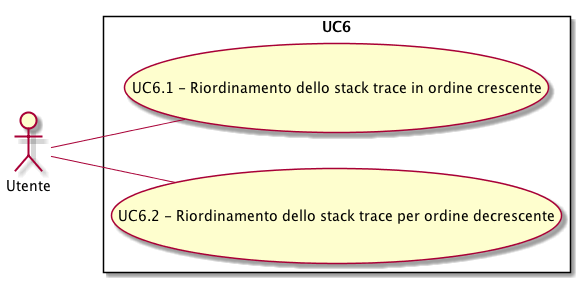
\includegraphics[scale=0.45]{./UC/UC6.png}
	\caption{Riordinamento della stack trace}\label{}
\end{figure}
\begin{itemize}
	\item \textbf{Attori}: Utente
	\item \textbf{Descrizione}: L'attore intende manipolare l'ordinamento dello stack trace.
	\item \textbf{Precondizione}: Deve essere stata visualizzata all'interno del plugin la stack trace.
	\item \textbf{Flusso principale degli eventi}: L'attore intende riordinare la stack trace e questa viene riordinata.
	
	\begin{itemize}
		\item Riordinamento dello stack trace in ordine crescente (UC6.1)
		\item Riordinamento dello stack trace per ordine decrescente (UC6.2)
	\end{itemize}
	\item \textbf{Postcondizione}: La stack trace viene riordinata.
\end{itemize}
\subsection{Caso d'uso UC6.1: Riordinamento dello stack trace in ordine crescente}
\begin{itemize}
	\item \textbf{Attori}: Utente
	\item \textbf{Descrizione}: L'attore vuole riordinare la lista delle trace in ordine crescente.
	\item \textbf{Precondizione}: Deve essere stata visualizzata all'interno del plugin la stack trace.
	\item \textbf{Flusso principale degli eventi}: L'attore vuole riordinare la stack trace in ordine crescente e questo avviene in seguito all'interazione con un componente grafico.
	\item \textbf{Postcondizione}: La stack trace viene riordinata in ordine crescente.
\end{itemize}
\subsection{Caso d'uso UC6.2: Riordinamento dello stack trace per ordine decrescente}
\begin{itemize}
	\item \textbf{Attori}: Utente
	\item \textbf{Descrizione}: L'attore vuole riordinare la lista delle trace in ordine decrescente.
	\item \textbf{Precondizione}: Deve essere stata visualizzata all'interno del plugin la stack trace.
	\item \textbf{Flusso principale degli eventi}: L'attore vuole riordinare la stack trace in ordine decrescente e questo avviene in seguito all'interazione con un componente grafico.
	\item \textbf{Postcondizione}: La stack trace viene riordinata in ordine decrescente.
\end{itemize}
\subsection{Caso d'uso UC7: Riordinamento stack trace per momento di inizio dell'esecuzione}
\begin{itemize}
	\item \textbf{Attori}: Utente
	\item \textbf{Descrizione}: L'attore vuole riordinare la lista delle trace in base al momento di inizio dell'esecuzione.
	\item \textbf{Precondizione}: Deve essere stata visualizzata all'interno del plugin la stack trace.
	\item \textbf{Flusso principale degli eventi}: L'attore vuole riordinare la stack trace in base al momento di inizio dell'esecuzione e questo avviene in seguito all'interazione con un componente grafico.
	\item \textbf{Postcondizione}: La stack trace viene riordinata in base al momento di inizio dell'esecuzione.
\end{itemize}
\subsection{Caso d'uso UC8: Riordinamento stack trace per tempo di esecuzione}
\begin{itemize}
	\item \textbf{Attori}: Utente
	\item \textbf{Descrizione}: L'attore vuole riordinare la lista delle trace in base al tempo di esecuzione.
	\item \textbf{Precondizione}: Deve essere stata visualizzata all'interno del plugin la stack trace.
	\item \textbf{Flusso principale degli eventi}: L'attore vuole riordinare la stack trace in base al tempo di esecuzione e questo avviene in seguito all'interazione con un componente grafico.
	\item \textbf{Postcondizione}: La stack trace viene riordinata in base al tempo di esecuzione.
\end{itemize}
\subsection{Caso d'uso UC9: Fallimento caricamento dati della stack trace}
\begin{itemize}
	\item \textbf{Attori}: Utente
	\item \textbf{Descrizione}: I dati relativi alla stack trace non possono essere caricati per un errore interno.
	\item \textbf{Precondizione}: Si verifica un errore nel caricamento dei dati.
	\item \textbf{Flusso principale degli eventi}: La richiesta dei dati relativi alla stack trace dell'applicazione monitorata non può essere soddisfatta, dunque viene visualizzato un messaggio di errore al posto della stack trace.
	\item \textbf{Postcondizione}: Al posto della stack trace viene visualizzato un messaggio di errore.
\end{itemize}
\subsection{Caso d'uso UC10: Visualizzazione call tree}
\begin{figure} [H]
	\centering
	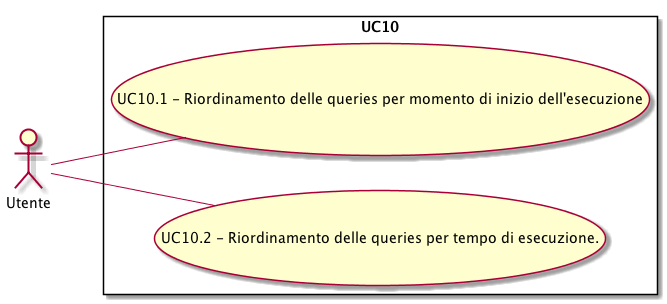
\includegraphics[scale=0.45]{./UC/UC10.png}
	\caption{Visualizzazione call tree}\label{}
\end{figure}
\begin{itemize}
	\item \textbf{Attori}: Utente
	\item \textbf{Descrizione}: L'attore intende visualizzare il call tree di una trace selezionata.
	\item \textbf{Precondizione}: Deve essere stato premuto un componente grafico adibito alla visualizzazione del call tree di una determinata trace.
	\item \textbf{Flusso principale degli eventi}: L'attore intende visualizzare il call tree di una determinata trace, quindi preme un componente grafico associato alla trace che ne determina la visualizzazione.
	\begin{itemize}
		\item Visualizzazione dettagli singolo metodo (UC10.1)
	\end{itemize}
	\item \textbf{Postcondizione}: Viene visualizzato il call tree della trace selezionata.
\end{itemize}
\subsection{Caso d'uso UC10.1: Visualizzazione dettagli singolo metodo}
\begin{figure} [H]
	\centering
	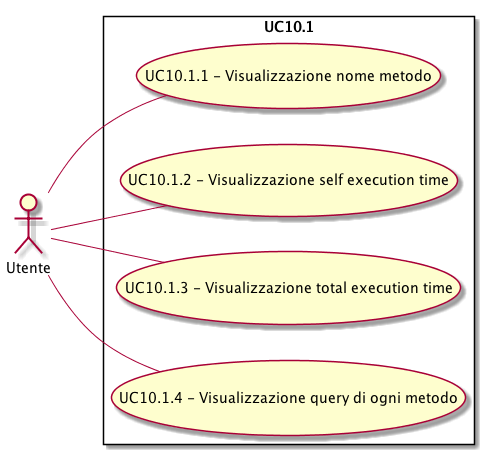
\includegraphics[scale=0.45]{./UC/UC10-1.png}
	\caption{Visualizzazione dettagli singolo metodo}\label{}
\end{figure}
\begin{itemize}
	\item \textbf{Attori}: Utente
	\item \textbf{Descrizione}: L'attore intende visualizzare per ogni metodo i relativi dettagli.
	\item \textbf{Precondizione}: Deve essere stato premuto un componente grafico adibito alla visualizzazione del call tree di una determinata trace.
	
	\item \textbf{Flusso principale degli eventi}: L'attore intende visualizzare, per ogni metodo, i relativi dettagli che vengono visualizzati e raggruppati in una riga della lista.
	\begin{itemize}
		\item Visualizzazione nome metodo (UC10.1.1)
		\item Visualizzazione self execution time (UC10.1.2)
		\item Visualizzazione total execution time (UC10.1.3)
		\item Visualizzazione query di ogni metodo (UC10.1.4)
	\end{itemize}
	\item \textbf{Postcondizione}: Vengono visualizzati i dettagli di ogni singolo metodo.
\end{itemize}
\subsection{Caso d'uso UC10.1.1: Visualizzazione nome metodo}
\begin{itemize}
	\item \textbf{Attori}: Utente
	\item \textbf{Descrizione}: L'attore intende visualizzare il nome di ogni metodo presente nel call tree.
	\item \textbf{Precondizione}: Deve essere stato caricato il call tree di una determinata trace.
	\item \textbf{Flusso principale degli eventi}: L'attore intende visualizzare il nome di ogni metodo presente nel call tree ed esso viene visualizzato forma testuale.
	\item \textbf{Postcondizione}: Per ogni metodo del call tree ne viene visualizzato il nome.
\end{itemize}
\subsection{Caso d'uso UC10.1.2: Visualizzazione self execution time}
\begin{itemize}
	\item \textbf{Attori}: Utente
	\item \textbf{Descrizione}: L'attore intende visualizzare il self execution time di ogni metodo presente nel call tree.
	\item \textbf{Precondizione}: Deve essere stato caricato il call tree di una determinata trace.
	\item \textbf{Flusso principale degli eventi}: L'attore intende visualizzare il self execution time di ogni metodo presente nel call tree ed esso viene visualizzato in forma testuale.
	\item \textbf{Postcondizione}: Per ogni metodo del call tree ne viene visualizzato il self execution time.
\end{itemize}
\subsection{Caso d'uso UC10.1.3: Visualizzazione total execution time}
\begin{itemize}
	\item \textbf{Attori}: Utente
	\item \textbf{Descrizione}: L'attore intende visualizzare il total execution time di ogni metodo presente nel call tree.
	\item \textbf{Precondizione}: Deve essere stato caricato il call tree di una determinata trace.
	\item \textbf{Flusso principale degli eventi}: L'attore intende visualizzare il total execution time di ogni metodo presente nel call tree ed esso viene visualizzato in forma testuale.
	\item \textbf{Postcondizione}: Per ogni metodo del call tree ne viene visualizzato il total execution time.
\end{itemize}
\subsection{Caso d'uso UC10.1.4: Visualizzazione query di ogni metodo}
\begin{itemize}
	\item \textbf{Attori}: Utente
	\item \textbf{Descrizione}: L'attore intende visualizzare le query effettuate da ogni metodo del call tree.
	\item \textbf{Precondizione}: Deve essere stato caricato il call tree di una determinata trace.
	\item \textbf{Flusso principale degli eventi}: Per ogni metodo del call tree l'attore intende visualizzare le query effettuate da esso, quindi ogni query viene visualizzata sotto il metodo che la ha eseguita.
	\item \textbf{Postcondizione}: Per ogni metodo del call tree vengono visualizzate le query da esso effettuate.
\end{itemize}
\subsection{Caso d'uso UC11: Cambio organizzazione della visualizzazione di un metodo del call tree}
\begin{figure} [H]
	\centering
	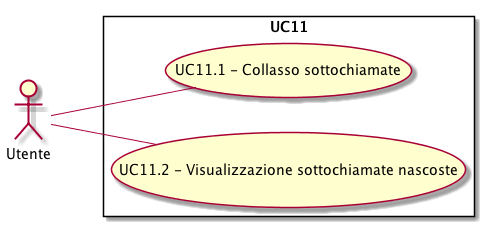
\includegraphics[scale=0.45]{./UC/UC11.png}
	\caption{Cambio organizzazione della visualizzazione di un metodo del call tree}\label{}
\end{figure}
\begin{itemize}
	\item \textbf{Attori}: Utente
	\item \textbf{Descrizione}: L'attore intende cambiare l'organizzazione della visualizzazione di un metodo e dei propri sottometodi attraverso dei componenti grafici.
	
	\item \textbf{Precondizione}: Deve essere stato caricato il call tree di una determinata trace.
	\item \textbf{Flusso principale degli eventi}: L'attore intende cambiare l'organizzazione della visualizzazione di un metodo del call tree, quindi preme un componente grafico che permette questo.
	\begin{itemize}
		\item Collasso sottochiamate (UC11.1)
		\item Visualizzazione sottochiamate nascoste (UC11.2)
	\end{itemize}
	\item \textbf{Postcondizione}: La visualizzazione di un metodo e dei suoi sottometodi viene cambiata.
\end{itemize}
\subsection{Caso d'uso UC11.1: Collasso sottochiamate}
\begin{itemize}
	\item \textbf{Attori}: Utente
	\item \textbf{Descrizione}: L'attore intende nascondere la lista delle sottochiamate eseguite da una singola chiamata all'interno del call tree.
	\item \textbf{Precondizione}: Il call tree di una trace deve essere stato visualizzato.
	\item \textbf{Flusso principale degli eventi}: L'attore clicca su un pulsante corrispondente alla chiamata della quale vuole nascondere le sottochiamate Le sottochiamate vengono nascoste.
	\item \textbf{Postcondizione}: Tutte le chiamate eseguite dalla singola chiamata vengono nascoste.
\end{itemize}
\subsection{Caso d'uso UC11.2: Visualizzazione sottochiamate nascoste}
\begin{itemize}
	\item \textbf{Attori}: Utente
	\item \textbf{Descrizione}: L'attore intende mostrare le sottochiamate nascoste di una specifica chiamata nel call tree.
	\item \textbf{Precondizione}: Devono essere state nascoste le sottochiamate.
	\item \textbf{Flusso principale degli eventi}: L'attore clicca su un pulsante corrispondente alla chiamata della quale vuole mostrare le sottochiamate Le sottochiamate vengono mostrate.
	\item \textbf{Postcondizione}: Vengono mostrate le sottochiamate di una chiamata.
\end{itemize}
\subsection{Caso d'uso UC12: Visualizzazione elenco delle query di una singola trace}
\begin{figure} [H]
	\centering
	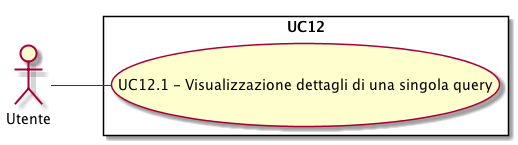
\includegraphics[scale=0.45]{./UC/UC12.png}
	\caption{Visualizzazione elenco delle query di una singola trace}\label{}
\end{figure}
\begin{itemize}
	\item \textbf{Attori}: Utente
	\item \textbf{Descrizione}: L'attore intende visualizzare tutte le query eseguite in una trace.
	\item \textbf{Precondizione}: Deve essere stato premuto un componente grafico adibito alla visualizzazione delle query di una determinata trace.
	\item \textbf{Flusso principale degli eventi}: L'attore richiede di visualizzare la lista di tutte le query eseguite da una trace quindi questa viene visualizzata.
	\begin{itemize}
		\item Visualizzazione dettagli di una singola query (UC12.1)
	\end{itemize}
	\item \textbf{Postcondizione}: Viene visualizzato l'elenco di tutte le query eseguite da una trace.
\end{itemize}
\subsection{Caso d'uso UC12.1: Visualizzazione dettagli di una singola query}
\begin{figure} [H]
	\centering
	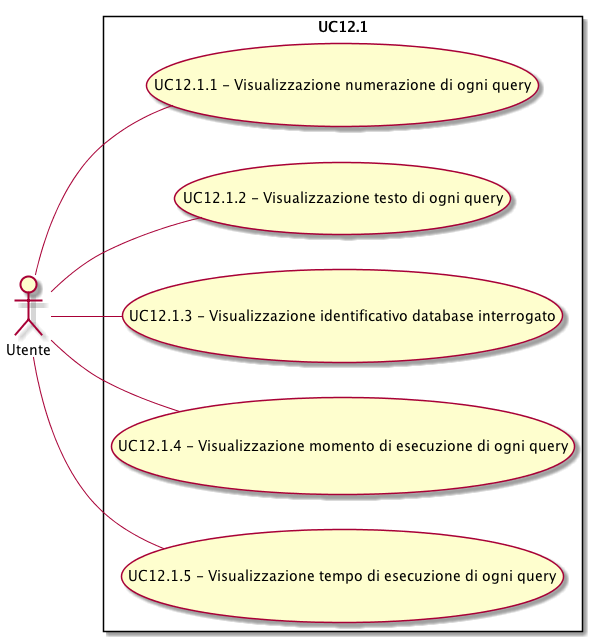
\includegraphics[scale=0.45]{./UC/UC12-1.png}
	\caption{Visualizzazione dettagli di una singola query}\label{}
\end{figure}
\begin{itemize}
	\item \textbf{Attori}: Utente
	\item \textbf{Descrizione}: L'attore intende visualizzare per ogni query i relativi dettagli.
	\item \textbf{Precondizione}: Deve essere stato premuto un componente grafico adibito alla visualizzazione delle query di una determinata trace.
	\item \textbf{Flusso principale degli eventi}: L'attore intende visualizzare, per ogni query, i relativi dettagli che vengono visualizzati e raggruppati in una riga della lista.
	\begin{itemize}
		\item Visualizzazione numerazione di ogni query (UC12.1.1)
		\item Visualizzazione testo di ogni query (UC12.1.2)
		\item Visualizzazione identificativo database interrogato (UC12.1.3)
		\item Visualizzazione momento di esecuzione di ogni query (UC12.1.4)
		\item Visualizzazione tempo di esecuzione di ogni query (UC12.1.5)
	\end{itemize}
	\item \textbf{Postcondizione}: Vengono visualizzati i dettagli di ogni singola query.
\end{itemize}
\subsection{Caso d'uso UC12.1.1: Visualizzazione numerazione di ogni query}
\begin{itemize}
	\item \textbf{Attori}: Utente
	\item \textbf{Descrizione}: L'attore intende visualizzare la lista delle query di una singola trace come un elenco numerato che parta da 1.
	\item \textbf{Precondizione}: Deve essere stato premuto un componente grafico adibito alla visualizzazione delle query di una determinata trace.
	\item \textbf{Flusso principale degli eventi}: L'attore intende visualizzare la lista delle query di una singola trace come un elenco numerato, quindi vicino ad ogni query viene disegnato un numero incrementale che parte da 1.
	\item \textbf{Postcondizione}: La lista delle query di una singola trace viene visualizzata come un elenco numerato.
\end{itemize}
\subsection{Caso d'uso UC12.1.2: Visualizzazione testo di ogni query}
\begin{itemize}
	\item \textbf{Attori}: Utente
	\item \textbf{Descrizione}: L'attore intende visualizzare il testo delle query nella lista delle query eseguite in una trace.
	\item \textbf{Precondizione}: Deve essere stato premuto un componente grafico adibito alla visualizzazione delle query di una determinata trace.
	\item \textbf{Flusso principale degli eventi}: L'attore intende visualizzare il testo delle query eseguite in una singola trace, dunque esso viene visualizzato.
	\item \textbf{Postcondizione}: Il testo di ogni query viene visualizzato nella lista.
\end{itemize}
\subsection{Caso d'uso UC12.1.3: Visualizzazione identificativo database interrogato}
\begin{itemize}
	\item \textbf{Attori}: Utente
	\item \textbf{Descrizione}: L'attore intende visualizzare l'identificativo del database interrogato da ogni query presente nella lista query eseguite in una trace.
	\item \textbf{Precondizione}: Deve essere stato premuto un componente grafico adibito alla visualizzazione delle query di una determinata trace.
	
	\item \textbf{Flusso principale degli eventi}: L'attore intende visualizzare l'identificativo del database interrogato dalla query e quando la lista viene caricata nel plugin questi vengono rappresentati in forma testuale.
	\item \textbf{Postcondizione}: Per ogni query nell'elenco viene visualizzato l'identificativo del database interrogato.
\end{itemize}
\subsection{Caso d'uso UC12.1.4: Visualizzazione momento di esecuzione di ogni query}
\begin{itemize}
	\item \textbf{Attori}: Utente
	\item \textbf{Descrizione}: L'attore intende visualizzare data e orario del momento in cui è iniziata l'esecuzione di ogni query.
	\item \textbf{Precondizione}: Deve essere stato premuto un componente grafico adibito alla visualizzazione delle query di una determinata trace.
	\item \textbf{Flusso principale degli eventi}: L'attore intende visualizzare data e orario del momento in cui è iniziata l'esecuzione di ogni query dunque tali informazioni vengono rappresentate in maniera testuale.
	\item \textbf{Postcondizione}: Vengono mostrate la data e l'orario del momento in cui è iniziata l'esecuzione di ogni query.
\end{itemize}
\subsection{Caso d'uso UC12.1.5: Visualizzazione tempo di esecuzione di ogni query}
\begin{itemize}
	\item \textbf{Attori}: Utente
	\item \textbf{Descrizione}: L'attore intende visualizzare il tempo di esecuzione di ogni query.
	\item \textbf{Precondizione}: Deve essere stato premuto un componente grafico adibito alla visualizzazione delle query di una determinata trace.
	\item \textbf{Flusso principale degli eventi}: L'attore intende visualizzare il tempo di esecuzione di ogni query ed esso viene rappresentato sotto forma di testo.
	\item \textbf{Postcondizione}: Per ogni query presente nella lista viene visualizzato il proprio tempo di esecuzione.
\end{itemize}
\subsection{Caso d'uso UC13: Riordinamento delle query di una singola trace}
\begin{figure} [H]
	\centering
	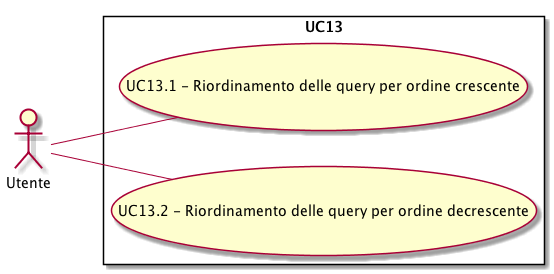
\includegraphics[scale=0.45]{./UC/UC13.png}
	\caption{Riordinamento delle query di una singola trace}\label{}
\end{figure}
\begin{itemize}
	\item \textbf{Attori}: Utente
	\item \textbf{Descrizione}: L'attore intende manipolare l'ordinamento delle query di una singola trace.
	\item \textbf{Precondizione}: Deve essere stata visualizzata la lista di query di una singola trace.
	\item \textbf{Flusso principale degli eventi}: L'attore intende riordinare le query di una singola trace e queste viene riordinata.
	\begin{itemize}
		\item Riordinamento delle query per ordine crescente (UC13.1)
		\item Riordinamento delle query per ordine decrescente (UC13.2)
	\end{itemize}
	\item \textbf{Postcondizione}: La lista di query relative ad una singola trace viene riordinata.
\end{itemize}
\subsection{Caso d'uso UC13.1: Riordinamento delle query per ordine crescente}
\begin{itemize}
	\item \textbf{Attori}: Utente
	\item \textbf{Descrizione}: L'attore vuole riordinare la lista delle query di una singola trace in ordine crescente.
	\item \textbf{Precondizione}: Deve essere stata visualizzata la lista di query di una singola trace.
	\item \textbf{Flusso principale degli eventi}: L'attore vuole riordinare la lista delle query di una singola trace in ordine crescente e questo avviene in seguito all'interazione con un componente grafico.
	\item \textbf{Postcondizione}: La lista delle query di una singola trace viene riordinata in ordine crescente.
\end{itemize}
\subsection{Caso d'uso UC13.2: Riordinamento delle query per ordine decrescente}
\begin{itemize}
	\item \textbf{Attori}: Utente
	\item \textbf{Descrizione}: L'attore vuole riordinare la lista delle query di una singola trace in ordine decrescente.
	\item \textbf{Precondizione}: Deve essere stata visualizzata la lista di query di una singola trace.
	\item \textbf{Flusso principale degli eventi}: L'attore vuole riordinare la lista delle query di una singola trace in ordine decrescente e questo avviene in seguito all'interazione con un componente grafico.
	\item \textbf{Postcondizione}: La lista delle query di una singola trace viene riordinata in ordine decrescente.
	
\end{itemize}
\subsection{Caso d'uso UC14: Riordinamento delle query per momento di inizio dell'esecuzione}
\begin{itemize}
	\item \textbf{Attori}: Utente
	\item \textbf{Descrizione}: L'attore vuole riordinare la lista delle query di una singola trace in base al momento di inizio dell'esecuzione.
	\item \textbf{Precondizione}: Deve essere stata visualizzata la lista di query di una singola trace.
	\item \textbf{Flusso principale degli eventi}: L'attore vuole riordinare la lista di query di una singola trace in base al momento di inizio dell'esecuzione e questo avviene in seguito all'interazione con un componente grafico.
	\item \textbf{Postcondizione}: La lista di query di una singola trace viene riordinata in base al momento di inizio dell'esecuzione.
\end{itemize}
\subsection{Caso d'uso UC15: Riordinamento delle query per tempo di esecuzione}
\begin{itemize}
	\item \textbf{Attori}: Utente
	\item \textbf{Descrizione}: L'attore vuole riordinare la lista delle query di una singola trace in base al tempo di esecuzione.
	\item \textbf{Precondizione}: Deve essere stata visualizzata la lista di query di una singola trace.
	
	\item \textbf{Flusso principale degli eventi}: L'attore vuole riordinare la lista di query di una singola trace in base al tempo di esecuzione e questo avviene in seguito all'interazione con un componente grafico.
	\item \textbf{Postcondizione}: La lista di query di una singola trace viene riordinata in base al tempo di esecuzione.
\end{itemize}
